\documentclass{article}
\usepackage{amsmath,bm}
\usepackage{amssymb}
\usepackage{amsfonts}
\usepackage[usenames]{xcolor}
\usepackage{graphicx}
\usepackage{epsf}
\usepackage{hyperref}
\usepackage{enumitem}

% \usepackage[LGR,T1]{fontenc}
% \usepackage[sfdefault]{FiraSans}
% \usepackage[nomap]{FiraMono}
% \usepackage[var0,varqu]{zi4}
% \renewcommand{\rmdefault}{zi4}
%\renewcommand{\sfdefault}{zi4}

\usepackage{unicode}

% titlepage causes separate title page
% our latex is biased off 1in vertically and horizontally
\newtheorem{theorem}{Theorem}
\setlength{\topmargin}{0.1in}
\setlength{\oddsidemargin}{0in}
\setlength{\evensidemargin}{0in}
\setlength{\headheight}{0in}
\setlength{\headsep}{0in}
\setlength{\textheight}{9in}
\setlength{\textwidth}{6.5in}
% require that floats fill 90% of a page in order for that page to be
% ``float-only''
\renewcommand{\dblfloatpagefraction}{0.9}
\renewcommand{\floatpagefraction}{0.9}
\newenvironment{bibparagraph}{\begin{list}{}{ %
    \setlength{\labelsep}{-\leftmargin} %
    \setlength{\labelwidth}{0pt} %
    \setlength{\itemindent}{-\leftmargin} %
    \setlength{\listparindent}{0pt}}}{\end{list}}
\def\makefigure#1#2{\begin{figure}
\begin{center}
\input{#1}
\end{center}
\caption{#2}
\label{#1}
\end{figure}}

\def\limplies{\; \supset \;}
\def\land{\: \wedge \:}
\def\lor{\: \vee \:}
\def\iff{\; \equiv \;}
\def\lnot{\neg}
\def\lforall#1{\forall \: #1 \;}
\def\lexists#1{\exists \: #1 \;}
\def\glitch#1{{\tt #1}} % glitch on
%\def\glitch#1{} % glitch off
\def\comment#1{}
\def\pnil{[\;]}
\def\pif{\; \mbox{\tt :- } \;}
\def\tuple#1{$\langle #1\rangle$}
\def\mtuple#1{\langle #1\rangle}
\def\ceiling#1{\lceil #1\rceil}
\def\floor#1{\lfloor #1\rfloor}
\def\centerps#1{\begin{center}
\leavevmode
\epsfbox{#1}
\end{center}}
\def\argmax{\mathop{\rm argmax}}
\def\argmin{\mathop{\rm argmin}}
\def\grad{\nabla\!}
\def\celsius{^\circ\mbox{C}}
%\long\def\answer#1{}  % comment out for solutions
%\long\def\question#1{#1} % comment out for solutions
\long\def\answer#1{\color{green!10!blue!90!}{\sf \noindent #1}
\vspace{2ex}}  % comment in for solution
\long\def\question#1#2{\color{black}\rm \noindent {#1}.) #2 \par \vspace*{2ex}
} % comment in for solution
%\renewcommand{\labelenumi}{(\alph{enumi})}
%\newcommand{\mbx}{\mathbf{x}}
\newcommand{\mb}[1]{{\mathbf{#1}}}

\def\x{{\bf x}}
\def\w{{\bf w}}
\def\y{{\bf y}}

\usepackage{array}
\def\arraystretch{2.0}%


\begin{document}

{\small
Submitted by: {Oluwasegun Somefun}, somefuno@oregonstate.edu
}
{\Large
\begin{center}
  AI534 ---  IA2 Homework Report {Due Oct 29th 11:59pm, 2021}
\end{center}
}

\section{Part 1: Ridge Regularization}
\question{a}{
  What trend do you observe for the training accuracy as we increase $\lambda$? Why is this
  the case? What trend do you observe for the validation accuracy? What is the best $\lambda$ value
  based on the validation accuracy?
}
\answer{
The training class accuracy remain approximately constant for a while, then generally reduces as we increase $\lambda \in \left[10^{-3}\hbox{, }10^{3}\right]$.
This is the case because, increase in $\lambda$, directly increase the loss function and hence approximation error.
The validation class accuracy also remain approximately constant for a while, then generally reduces as we increase $\lambda$ within the given range.
The best value in this range is $\lambda=10^{-3}$. This is illustrated in Figure~{\ref{figa}}
\begin{figure}[!ht]
  \centering
  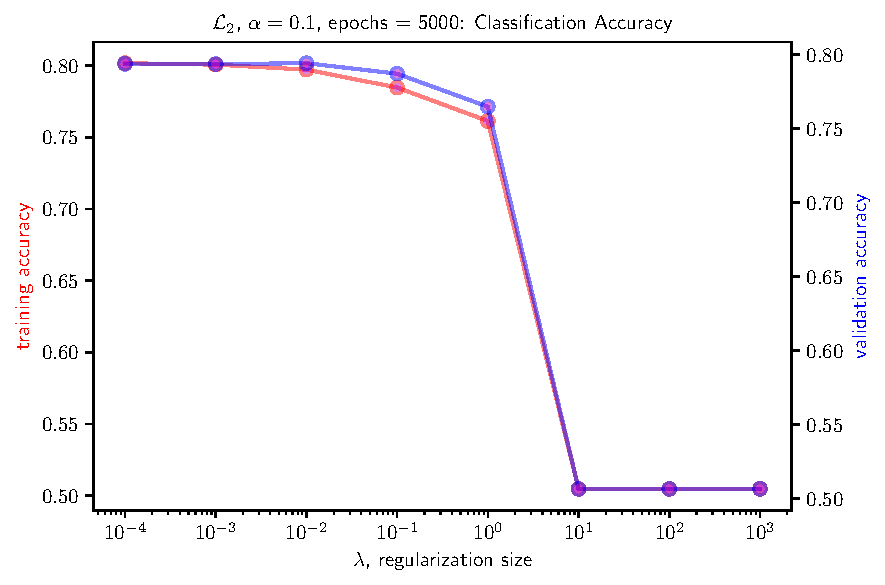
\includegraphics[width=0.8\linewidth]{figs/L2_trainvalcmp_plt.pdf}
  \caption{Comparison: class accuracy vs $\lambda$ }\label{figa}
\end{figure}

}

\question{b}{
  Do you see differences in the selected top features with different $\lambda$ values? What is
  your explanation for this behavior?
}
\answer{
The resulting top five features with respect to their weight magnitude 
are illustarated below with $\lambda^{*}=10^{-3}$, $\lambda_{+}=10^{-4}$ and
$\lambda_{-}=10^{-2}$ in Table~\ref{tab1}. 
Interestingly, in this range there is no much difference in the 
selected top 5 features. However, as the value of $\lambda$ increases 
outside this range, the top features, gradually begin to differ.
\begin{table}[!ht]
  \fontsize{10}{10} \centering \sf 
  \caption{$\mathcal{L}_2$: Features (Top-5) with largest $|\mathbf{\omega}|$}
  \vspace{2ex}
  \begin{tabular}{|c|c|>{\bfseries}c|c|}
    \hline
    \textbf{Feature}            & $10^{-4}$ & $10^{-3}$ & $10^{-2}$ \\ \hline\hline
    Previously\_Insured         & -3.2264   & -2.9705   & -2.0701   \\\hline
    Vehicle\_Damage             & 2.2457    & 2.2035    & 1.9445    \\\hline
    Policy\_Sales\_Channel\_160 & -1.8431   & -1.6671   & -1.3914   \\\hline
    dummy                       & -1.0862   & -1.1732   & -0.9030   \\\hline
    Policy\_Sales\_Channel\_152 & -0.8891   & -0.8424   & -0.6267   \\ \hline
  \end{tabular}
  \label{tab1}
\end{table}
This can be interpreted as automatic feature mapping during the regression process. 
The optimization process automatically associates the most important features with larger weights
relative to the other features.
}


\question{c}{
  What trend do you observe for the sparsity of the model as 
  we change $\lambda$? 
  If we further increase $\lambda$, what do you expect? Why?
}
\answer{
  It can be observed from Figure~\ref{figb}, that as we change $\lambda$, 
  the model sparsity increases. Increase in $\lambda$ numerically forces the weights to be very close to zero.
  As $\lambda$ is increased further, we expect the model sparsity 
  to remain constant at a value equal or close to the number of features, which is $197$ in this case.
  \begin{figure}[!ht]
    \centering
    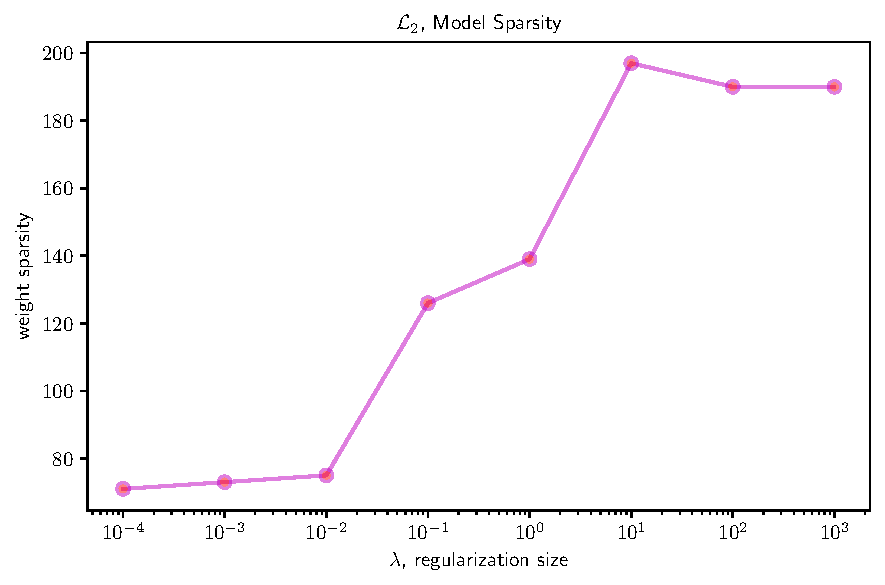
\includegraphics[width=0.8\linewidth]{figs/L2_sparsityplt.pdf}
    \caption{Model Sparsity vs $\lambda$ }\label{figb}
  \end{figure}
}


\section{Part 2: Lasso Regularization}
\question{a}{
  What trend do you observe for the training accuracy as we increase $\lambda$? Why is this
  the case? What trend do you observe for the validation accuracy? What is the best $\lambda$ value
  based on the validation accuracy?
}
\answer{
The training class accuracy remain approximately constant for a while, then generally reduces as we increase $\lambda \in \left[10^{-3}\hbox{, }10^{3}\right]$.
This is the case because, increase in $\lambda$, directly increase the loss function and hence approximation error.
The validation class accuracy also remain approximately constant for a while, then generally reduces as we increase $\lambda$ within the given range.
The best value in this range is $\lambda=10^{-3}$. This is illustrated in Figure~{\ref{figc}}
\begin{figure}[!ht]
  \centering
  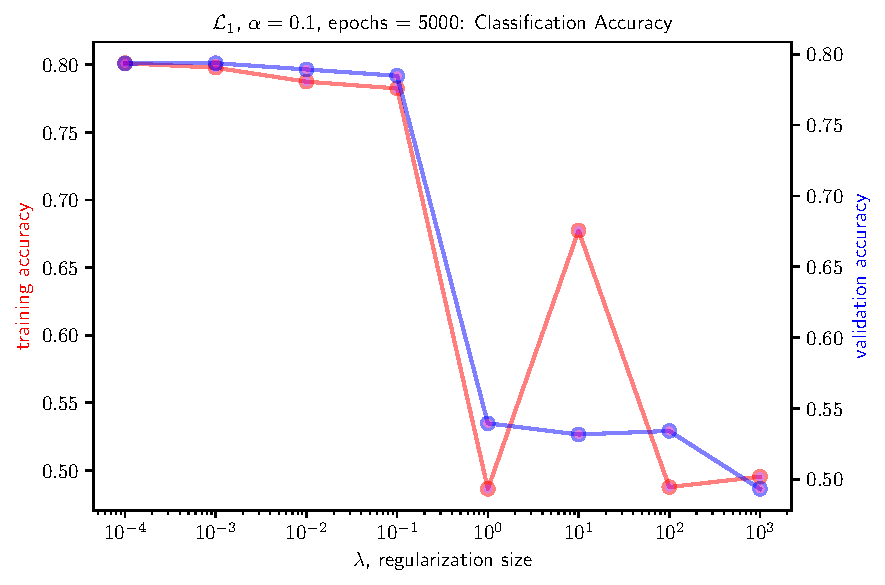
\includegraphics[width=0.8\linewidth]{figs/L1_trainvalcmp_plt.pdf}
  \caption{Comparison: class accuracy vs $\lambda$ }\label{figc}
\end{figure}

}

\question{b}{
  Do you see differences in the selected top features with different $\lambda$ values? What is
  your explanation for this behavior?
}
\answer{
The resulting top five features with respect to their weight magnitude 
are illustarated below with $\lambda^{*}=10^{-3}$, $\lambda_{+}=10^{-4}$ and
$\lambda_{-}=10^{-2}$ in Table~\ref{tab2}. 
Interestingly, in this range there is no much difference in the 
selected top 5 features. However, as the value of $\lambda$ increases 
outside this range, the top features, gradually begin to differ.
\begin{table}[!ht]
  \fontsize{10}{10} \centering \sf 
  \caption{$\mathcal{L}_1$: Features (Top-5) with largest $|\mathbf{\omega}|$}
  \vspace{2ex}
  \begin{tabular}{|c|c|>{\bfseries}c|c|}
    \hline
    \textbf{Feature}            & $10^{-4}$ & $10^{-3}$ & $10^{-2}$ \\ \hline\hline
    Previously\_Insured         & -3.2506   & -3.1560   & -2.5235   \\\hline
    Vehicle\_Damage             & 2.2440   & 2.2261   & 2.0939    \\\hline
    Policy\_Sales\_Channel\_160 & -1.8596   & -1.8089   & -1.2236   \\\hline
    dummy                       & -1.1046   & -1.2292   & -1.0126   \\\hline
    Policy\_Sales\_Channel\_152 & -0.9008   & -0.9347   & -0.7326   \\ \hline
  \end{tabular}
  \label{tab2}
\end{table}
This can be interpreted as automatic feature mapping during the regression process. 
The optimization process automatically associates the most important features with larger weights
relative to the other features.
}


\question{c}{
  What trend do you observe for the sparsity of the model as 
  we change $\lambda$? 
  If we further increase $\lambda$, what do you expect? Why?
  Is this trend different from what you observed in 1(c)?
Provide your explanation for your observation.
}
\answer{
  It can be observed from Figure~\ref{figd}, that as we change $\lambda$, 
  the model sparsity trend is irregular. We expect that an increase in $\lambda$ numerically forces the weights to be very close to zero.
  As $\lambda$ is increased further, we expect the model sparsity 
  to remain constant at a value equal or close to the number of features, which is $197$ in this case.
  However, compared to the observations in 1c, the expected sparsity trend seems not to be the case.
  The reason may be due to the discontinous nature of lasso regularization.

  \begin{figure}[!ht]
    \centering
    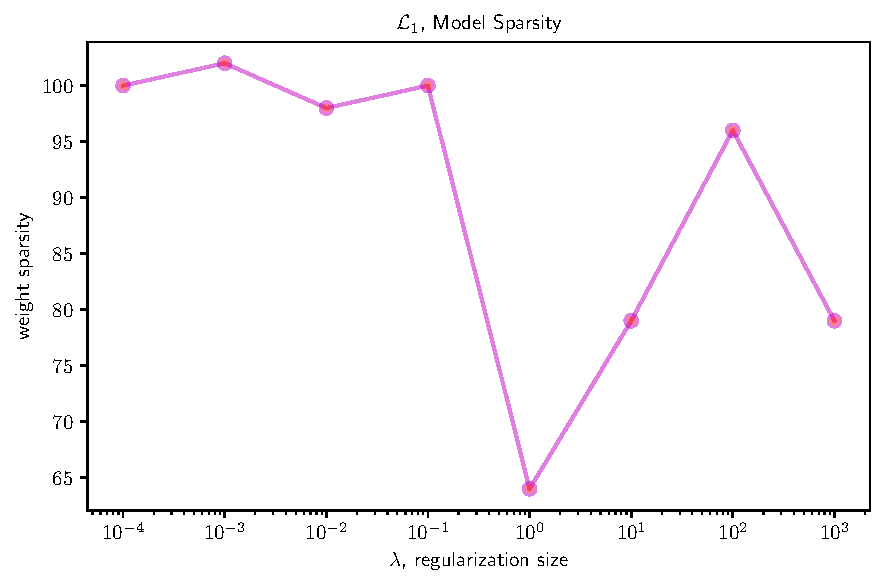
\includegraphics[width=0.8\linewidth]{figs/L1_sparsityplt.pdf}
    \caption{Model Sparsity vs $\lambda$ }\label{figd}
  \end{figure}
}

\section{Part 3: Kaggle Competition}
\question{a}{
  For this part, you need to describe the methods you used and their performance on the public
leaderboard. How do you handle the data usage? Do you treat the features differently from
what was used for Part 1 and 2? What do you think is limiting the performance you can get
on this dataset? The amount of data? the availability of features? the complexity of the
algorithm?
}
\answer{
  The approach to this part is outlined below:

  \textbf{Methods}

  Learning rate: $\alpha=0.1$, 

  Ridge-regularization: $\lambda=[10^{-4}\hbox{, }10^{-3}]$ 

  Epochs: $[2500, 10000]$
  
  Training was performed on a combined data of the train and dev datasets. 
  The performance on the test-data seems to increase using the listed set-up above, with a balanced fitting found within the mid-range of the 
  Epochs and $\lambda$-value listed above.
  
  \textbf{Data Preprocessing}: The three numeric features in the dataset have low correlation with the \textbf{Response} class,
  so they were dropped.

  \textbf{Comments}: Using logistic regression, the limiting performance out of this dataset 
  may be due to the nature of the dataset itself, allowing a small local area of global convergence to a classification accuracy around 80\%.
}



\end{document}